%documentclass[twocolumn]{report}
\documentclass{scrbook}
\usepackage[british]{babel}
\usepackage{graphicx}
\usepackage{float}
\usepackage{hyperref}
\usepackage{caption}
\usepackage[usenames,dvipsnames]{xcolor}
\usepackage{subfigure}
\floatstyle{boxed}
\usepackage{listings}
\lstloadlanguages{C++}
\lstset{
	rulecolor=,
	language=matlab,
  basicstyle=\scriptsize,
  upquote=true,
  aboveskip={1.5\baselineskip},
  columns=fixed,
  showstringspaces=false,
  extendedchars=true,
  breaklines=true,
  prebreak = \raisebox{0ex}[0ex][0ex]{\ensuremath{\hookleftarrow}},
  frame=single,
  showtabs=false,
  showspaces=false,
  showstringspaces=false,
  identifierstyle=\ttfamily,
  keywordstyle=\color[rgb]{0,0,1},
  commentstyle=\color[rgb]{0.133,0.545,0.133},
  stringstyle=\color[rgb]{0.627,0.126,0.941},
  language=C++
}
\usepackage{wrapfig}
\usepackage{keystroke}
\usepackage{tikz}
\usetikzlibrary{calc}

\newfloat{program}{htb}{lop}

%\lstset{frameround=fttt}
\newfloat{program}{H}{lop}
\renewcommand{\textfraction}{0.05}
\renewcommand{\topfraction}{0.95}
\renewcommand{\bottomfraction}{0.95}
\renewcommand{\floatpagefraction}{0.35}
\setcounter{totalnumber}{5}

\newcommand{\HRule}{\rule{\linewidth}{0.5mm}}
\newcommand{\libbats}{{\tt libbats} }

%\author{Little Green BATS}
\title{Libbats Manual}

\begin{document}

\frontmatter

\begin{titlepage}
{\noindent
\vspace{2cm}\\
\textbf{
{\texttt{\Huge libbats}}\\[0.5cm]
{\textsf{\Huge User Manual}}\\[2.5cm]
}
%\HRule \\[0.5cm]
 \textbf{\textsf{\Large Little Green BATS}}\\
 {\sf\large University of Groningen, the Netherlands}\\[0.5cm]
% {\large\url{http://www.littlegreenbats.nl}}\\
 \textbf{\textsf{\Large Bold Hearts}}\\
 {\sf\large University of Hertfordshire, UK}\\
 {\large\url{http://homepages.herts.ac.uk/~epics/boldhearts}}\\[0.5cm]
\vfill
\begin{center}
{\sf\large v. 3.0.1}
\end{center}
}
\end{titlepage}

\tableofcontents

%\include{_introduction}
\chapter{Introduction}

If you read this, you will probably already know about the RoboCup
initiaive: to progress robotics and artificial intelligence through
competition, to such a level that in 2050 an artificial football team
can beat the human world champions. Several leagues exist to focus on
seperate aspects of this problem, of which the 3D Soccer Simulation
(Sub) League is one. The aim of this league is to develop team
strategies and behaviors that are not (yet) feasible in the hardware
leagues.

This is the manual of \libbats, a library that can be used to get
started in the RoboCup 3D Simulation. It was originally developed by
the RoboCup 3D Simulation team the Little Green BATS in
2006. Currently it is being maintained and used in competitions by the
BATS and by team Bold Hearts, both vice world champion teams (in 2007
and 2009 respectively). This library can freely be used, both as in
free beer and free speech, to create your own (team of) RoboCup 3D
simulation agent(s) and to do research and enter competitions with. It
supplies some modules to get you started quickly, is generic enough to
add any algorithm, behavior model or learning method and still gives
you detailed control of the basics if required.

This manual is intended to give you an overview of the library and to
get you familiar with the structure and use of its parts. You can have
your own agent running within a few lines of code. More detailed
information on all possibilities can be found in the documentation in
the source code. If you want you can dig through all this code, but we
suggest to install doxygen
\footnote{\url{http://www.stack.nl/~dimitri/doxygen/}} instead. If you
do this and follow the installation instructions in chapter
\ref{chInstallation}, you will find this documentation nicely
formatted with HTML in the {\tt docs/html} directory.

The next chapter will give a brief discussion of the
SimSpark/RCSSServer3D simulation environment, which is used in the 3D
Soccer Simulation, and the way an agent should interact with it. This
chapter can in theory be skipped, since \libbats offers abstractions
and tools such that you don't have to worry about low level
issues. However, a general understanding of these will probably be
beneficial anyway.

After that we will give a tutorial of how to install the simulation
environment and \libbats, and some configuration options. Chapter
\ref{chQuickstart} takes you through the steps of creating your first
agent and shows how easy it is to set up a new team using
\libbats. The next chapters will go into the different parts and
modules of \libbats in more depth.

If something is still unclear, you found a bug or just have a question
related to this library, do not hesitate to contact us, preferably
through \libbats' Launchpad
page\footnote{\url{http://launchpad.net/littlegreenbats}}. Good luck
and happy coding!

\mainmatter


\chapter{SimSpark and RCSSServer3D}
\label{chSimspark}

This chapter offers a brief introduction of the simulation architecture used in the Robocup 3D Soccer Simulation competitions. The aim of this is to give a global understanding of the inner workings of the system; some details will be skipped, and even then a large part of this information is not necessarily needed to be able to create a team using {\tt libbats}. However, a more fundamental understanding can help a great deal to see what is going on. For a more in-depth treatment, see the SimSpark wiki at \url{http://simspark.sourceforge.net/wiki}.

\section{Basic Architecture}


The RoboCup 3D Soccer Simulation competitions use a unified simulation platform, SimSpark/RCSSServer3D, to supply the simulation of the soccer field, robot mechanics, game rules, etc. In 2006-2007 the first versions of SimSpark were developed, as a generic physics/robotics simulator, with a specific implementation for RoboCup 3D Soccer Simulation. Later on these two parts were explicitly separated: SimSpark now just includes the basic simulation engine, which takes care of the low level physics simulation and interfacing with agents, and exposes several templates to implement specific robot models, visualization systems and a plug-in system. The collection of implementations and plug-ins specific for the RoboCup 3D Simulation league is placed in the separate RCSSServer3D (RoboCup Soccer Simulation Server 3D) package. Together they form what is commonly referred to as '\emph{the simulation server}', '\emph{the simulator}', or '\emph{the server}'.

As said, the simulator takes care of all the world and game aspects. It also supplies a fixed physical robot model, which is the same for each agent an all teams. The simulator determines which sensor information is available for each robot at each time step and executes control commands supplied by the robot's 'brain'. This brain is what a team, i.e. you, has to create in order to be able to participate in the RoboCup 3D Soccer Simulation.

The brain of a robot consists of a standalone program and is connected to its body through a TCP/IP connection; the simulator opens a port (by default 3100), to which your program can connect. After some handshaking messages (explained below), the server will send sensor information at each time step (by default every 0.02 seconds). In reaction to such a sensor message your agent should send a control message, before the end of the time step. This message contains control commands for the agent's controllers, in our case these are target angular velocities for the robot's joints. This perception-action loop is represented in Fig.~\ref{fig:simulator}. This figure also shows that the physics simulation and the visualization of the results of this simulation are separated; the server opens another port (by default 3200), to which a so called '\emph{monitor}' can connect. Through this connection the server sends all information needed by a monitor to make a graphical representation of the current state of the simulation. The monitor in its turn can send commands to the server to control the simulation, which is done for instance when starting the game with a kick off.

\begin{figure}[t]
\begin{center}
	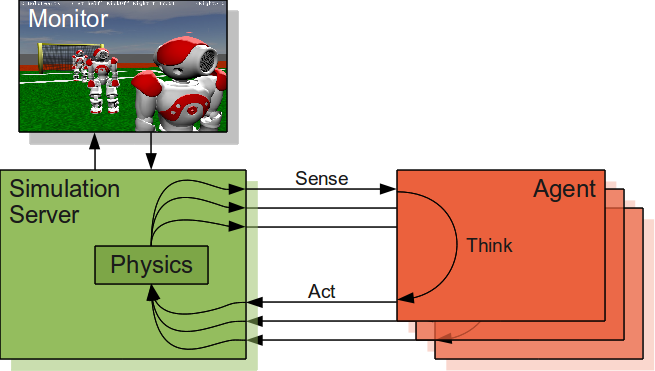
\includegraphics[width=0.70\textwidth]{simulator}
	\captionof{figure}{Interactions between simulator, monitor and agents. Each box represents a stand alone program, arrows between boxes depict the TCP/IP connections used for communication.}
	\label{fig:simulator}
\end{center}
\end{figure}

The communication between the server and the agents and between the server and a monitor follows a Lisp-like protocol, in which messages contain \emph{predicates} in the form of {S-expressions}. A predicate consists of a list of elements, the first of which is the name and the rest are its parameters. These parameters can again be predicates, resulting in a tree of predicates. As a simple example, the statement ``the current game mode number is 6'' is contained in the message {\tt (playMode 6)}. A more extensive example, taken from an actual simulation run, is given in Fig.~\ref{fig:sensemsg}. In the next section we will give an explanation of the different predicates.

\begin{figure}[t]
\begin{center}
\texttt{\small
(\textcolor{Red}{(time (now 70.32))} \textcolor{Blue}{(GS (t 0.00) (pm BeforeKickOff))} \textcolor{Brown}{(GYR (n torso) (rt -0.12 0.13 -0.01))} \textcolor{OliveGreen}{(ACC (n torso) (a -0.06 -0.06 9.81))} \textcolor{Purple}{(HJ (n hj1) (ax 0.00)) (HJ (n hj2) (ax 0.00))} \textcolor{Orange}{(See (G2R (pol 17.64 -12.45 1.00)) (G1R (pol 17.30 -5.75 0.93)) (F1R (pol 17.50 10.54 -1.74)) (F2R (pol 19.35 -26.93 -1.46)) (B (pol 8.69 -18.65 -3.10)) (P (team Enemy) (id 2) (head (pol 15.79 -15.79 0.06)) (rlowerarm (pol 15.75 -15.57 -0.84)) (llowerarm (pol 15.85 -15.84 -0.49)) (rfoot (pol 15.79 -15.37 -1.64)) (lfoot (pol 15.79 -16.08 -1.91))))} \textcolor{Purple}{(HJ (n raj1) (ax 90.00)) (HJ (n raj2) (ax -64.10)) (HJ (n raj3) (ax -0.00)) (HJ (n raj4) (ax -0.03)) (HJ (n laj1) (ax 90.00)) (HJ (n laj2) (ax 64.10)) (HJ (n laj3) (ax -0.00)) (HJ (n laj4) (ax 0.04)) (HJ (n rlj1) (ax 0.01)) (HJ (n rlj2) (ax -0.05)) (HJ (n rlj3) (ax 0.01)) (HJ (n rlj4) (ax -0.00)) (HJ (n rlj5) (ax 0.02)) (FRP (n rf) (c 0.02 -0.03 -0.01) (f 0.19 0.08 21.04)) (HJ (n rlj6) (ax 0.08)) (HJ (n llj1) (ax 0.00)) (HJ (n llj2) (ax 0.01)) (HJ (n llj3) (ax -0.00)) (HJ (n llj4) (ax -0.00)) (HJ (n llj5) (ax 0.03)) (FRP (n lf) (c -0.01 -0.03 -0.02) (f -0.02 0.11 24.22)) (HJ (n llj6) (ax 0.00))})
}
	\captionof{figure}{Example message sent by the server to an agent. Red: time, blue: game state, brown: gyroscopic sensor, green: accelerometer, purple: joint angles, orange: vision.}
	\label{fig:sensemsg}
\end{center}
\end{figure}

\section{Protocol}

Here we will give a small example of a proper communication sequence between an agent and the simulator.

\begin{description}
	\item[Connect] Of course, first of all the agent should connect to the agent port of the server, by default port number 3100.
	\item[Create] After connection, the agent should ask the simulator to create a new robot model for it. This is done with a {\tt scene} predicate, which takes the name of a Ruby Scene Graph (RSG) file that contains the model's description as an argument. Currently, the 3D Simulation League uses a model based on the Nao robot:
	
	{\tt (scene rsg/agent/nao/nao.rsg)}
	\item[Initialize] The server will now start sending messages to the agent. However, before doing anything else, the agent has to finalize its initialization. It has to tell the simulator from which team it is and what uniform number ('\emph{unum}') it wants, by sending an {\tt init} predicate:
	
	{\tt (init (unum 2)(teamname MyTeam))}
	
	If unum 0 is sent, the simulator will appoint the next free uniform number to the agent. In response to this message, the simulator will reply with a message containing confirmation of the uniform number selected by the agent, or chosen by the simulator, and on which side of the field, left or right, the agent's team plays:
	
	{\tt ((time (now 5.80)) \textcolor{Red}{(GS (unum 2) (team left) (t 0.00) (pm BeforeKickOff))} (GYR (n torso) (rt -0.00 0.00 0.00)) (ACC (n torso) (a 0.00 0.00 9.81)) (HJ (n hj1) (ax -0.00))... }
	
	This completes the initial handshake sequence.
	
	\item[Sense] From now on, the simulator sends messages containing time, game state and perceptor information at each time step. You have already seen an example of these in Fig.~\ref{fig:sensemsg}. These senses consist of the state of several internal sensors, namely a gyroscopic and an accelerometric sensor measuring the agen's torso angular velocity and linear acceleration respectively, and two pressure sensors on the feet, and of visual data. This visual data contains the coordinates of objects in the field of view of the agent, i.e. the ball, several body parts of other agents, corner flags and goal posts, and lines. The field of view of an agent is by default 120 degrees both horizontally as vertically.
	
	\item[Act] After each simulator message, the agent should reply with an action message. Such a message contains control commands for the agent's actuators, i.e. a target angular velocity for each joint. For instance, the following message tells the simulator to move the two head joints {\tt he1} and {\tt he2}, and the first joints of both arms, {\tt lae1} and {\tt rae2}\footnote{SimSpark's communication protocol measures angles in degrees. Note however that {\tt libbats} internally uses radians, (and radians per second for angular velocities).}:
	
	{\tt (he1 11.759) (he2 -8.4038) (lae1 -18.987) (rae1 -18.985)}
	
	If for some joints no control is specified, the last target angular velocity that was sent is used by the simulator. Besides the joint actuators, there is a special 'beam' actuator, that can be used to quickly position an agent before kick-offs. It takes as arguments the x and y coordinates to beam to and the angle to face at. So, to beam to coordinates (-7, 1.5), while face angle 0, which is towards the opponent's goal, the agent should send the following message:
	
	{\tt (beam -7 1.5 0)}
	
\end{description}

%\section{Robot Model}

%The agent model used in the RoboCup 3D Soccer Simulation competitions is of a humanoid robot, roughly based on Aldeberan's Nao robot, shown 

\chapter{Installation}
\label{chInstallation}

This section describes the installation procedure for the RoboCup 3D
Simspark simulation server and for the \libbats library.

\section{RoboCup 3D Simspark Simulation Server}

For the latest installation instructions of the simulator, see the SimSpark project's wiki: \\
\url{http://simspark.sourceforge.net/wiki}\\
There you will find instructions for installation on various Linux
distributions, as well as for Windows and MacOS.

\section{libbats}

\begin{description}
\item[Dependencies] Install the necessary dependencies. For Ubuntu,
  and possibly other Debian based distributions, run:
\begin{verbatim}
$ sudo apt-get install libxml2-dev libsigc++-2.0-dev libgtkmm-2.4-dev
\end{verbatim}
  On Arch, run as root:
\begin{verbatim}
$ pacman -S libxml2 libsigc++ gtkmm
\end{verbatim}
  You can leave out {\tt gtkmm} if you don't want to build the GTK
  based debugger implementation.
\item[libbats] Install the latest version of {\tt libbats}:
  \begin{enumerate}
  \item Download the latest source code package release from: \\
    \url{https://github.com/sgvandijk/libbats/releases}
  \item Unpack and navigate to the source code directory:
\begin{verbatim}
$ tar xvzf libbats-x.y.z.tar.gz
$ cd libbats-x.y.z
\end{verbatim}
  \item Use CMake to configure, then make and install:
\begin{verbatim}
$ mkdir build && cd build
$ cmake ..
$ make
$ sudo make install
\end{verbatim}
  \end{enumerate}
\end{description}

\section{RoboViz}

RCSSServer3D comes with a monitor, RCSSMonitor3D, however it is rather
basic, both graphically as functionally. We suggest using RoboViz
instead, which offers much better visualization, and an advanced
debugging interface that is supported by \libbats. Installation
instructions for RoboViz can be found at:\\
\url{https://sites.google.com/site/umroboviz/}

\section{Testing}

To test whether everything is working correctly, start the simulator
with:
\begin{verbatim}
$ rcssserver3d
\end{verbatim}
This command should give you a greeting saying something similar to
the following:
\begin{verbatim}
rcssserver3d (formerly simspark), a monolithic simulator 0.6.5
Copyright (C) 2004 Markus Rollmann, 
Universität Koblenz.
Copyright (C) 2004-2009, The RoboCup Soccer Server Maintenance Group.

Type '--help' for further information
\end{verbatim}
plus some initialization output. This output will contain some
messages such as `{\tt ERROR: cannot find TextureServer}' and `{\tt
  ERROR: no FPSController found at}\\{\tt
  '/usr/scene/camera/physics/controller'}'; you can ignore these
messages.

Next start RoboViz. Change to the directory containing RoboViz' binary
and run:
\begin{verbatim}
./roboviz.sh
\end{verbatim}
After some time in which RoboViz connects to the server and
initializes its graphics a green field will appear with some lines and
two goals. Ta-da, you are successfully running the simulator! If
RoboViz reports 'Disconnected', you are not and something went wrong
with installing the simulator; see below for some troubleshooting
tips.

Finally start the example agent supplied with \libbats; in the
\libbats build directory execute:
\begin{verbatim}
$ cd examples/helloworld
$ ./helloworld
\end{verbatim}
If everything went well, an agent should appear, standing in the left
side of the field, waving its arms. You can also try another, more
advanced example agent; again, in the \libbats build directory, run:
\begin{verbatim}
$ cd examples/dribble
$ ./dribble
\end{verbatim}
This should start an agent which, when you start the game, walks to
the ball and dribbles it over to the opponent's goal.

\section{Troubleshooting}
\begin{enumerate}
\item To uninstall Simspark or RCSSServer3D, simply execute the
  following command within the respective build directory:
\begin{verbatim}
$ sudo make uninstall
\end{verbatim}
\item If compilation fails due to missing dependencies, as reported
  when running {\tt cmake} for the simulator or for
  \libbats, try looking up the required libraries using your
  distributions's package manager. For Ubuntu:
\begin{verbatim}
$ sudo apt-cache search <missing package>
\end{verbatim}
  For Arch:
\begin{verbatim}
$ pacman -Ss <missing package>
\end{verbatim}
\item Please refer to the SimSpark wiki for more information on how to
  install (or use) simspark, e.g. when using a different operating
  system:\\
  \url{http://simspark.sourceforge.net/wiki/index.php/Main_Page}.
\item Search through the sserver-three-d mailing list to see if there
  is a solution to your problem:\\
  \url{http://sourceforge.net/search/?type_of_search=mlists&group_id=24184}\\
  otherwise post it to the list (see
  \url{http://sourceforge.net/mail/?group_id=24184}).
\item For problems with \libbats, see the GitHub Issues section at: \\
  \url{https://github.com/sgvandijk/libbats/issues}.
\end{enumerate}

%%% Local Variables: 
%%% mode: latex
%%% TeX-master: "libbatsmanual"
%%% End: 

%\chapter{Running the Simulation}

\section{Starting}
To start the simulation server, run the following:
\begin{verbatim}
$ rcssserver3d
\end{verbatim}
This will generate some output to the terminal, including a list of 'not found' and 'Unknow function' errors. These are actually more like warnings and can be ignored. Next, you will have to start a monitor to be able to see what is going on in the simulation. If you run the monitor on te same machine as the simulator, use:
\begin{verbatim}
$ rcssmonitor3d
\end{verbatim}
If you run the monitor on a different machine, which can boost the speed of the simulator if you experience lag, use:
\begin{verbatim}
$ rcssmonitor3d --server 192.168.1.2
\end{verbatim}
Of course, use the actual address of the machine you run the server on. You can connect as many monitors you want (and your machine(s) can handle).

For convenience, there is also a script that starts both the server and the monitor, and kills the server when you close the monitor:
\begin{verbatim}
$ rcsoccersim3d
\end{verbatim}

\section{Controls}

\begin{center}
	\begin{tabular}{ll}
		\keystroke{1}-\keystroke{7} & Move camera to default positions \\
		\LArrow, \UArrow, \DArrow, \RArrow & Move camera horizontally \\
		\PgUp, \PgDown & Move camera vertically \\
		Click + drag & Turn camera \\
		\keystroke{K} & Kick-off \\
		\keystroke{B} & Drop ball \\
		\keystroke{L} & Free kick for the left team \\
		\keystroke{R} & Free kick for the right team \\
		\keystroke{Q} & Quit \\
	\end{tabular}
	\label{tab:}
\end{center}

%\chapter{SimSpark Simulation 3D Server}
\label{chServer}

The simulation is generated by the SimSpark Soccer Simulation Server. Agents can enter
the simulation by communicating with the soccer server using tcp sockets and a
hierarchical parentheses based communication protocol (think of LISP). The simulation maintains a
physically realistic (although at the moment noiseless) world, existing of a
soccer field and soccer(ro)bots. One agent program represents one soccer robot in the
simulation.

As of the World Championship of 2007 the simulation can only reliably run two agents per
team and still has some hiccups in the form of physics errors causing exploding body parts.
But we are confident that these will be resolved in the near future.

If you want to learn more you can take a look at the user manual for the server, but it is not quite finished yet:\\
\url{http://sourceforge.net/apps/mediawiki/sserver/index.php?title=Users_Manual}

\section{The Soccer Field}

Currently the actual size of the Soccer Field is unknown. In each corner resides a flag and on each side are two goal
posts. The size of the field is subjected to change and probably will not stay the same for
very long. Luckily the server notifies the agent of the size of the field at the initiation of communication.

\section{The Soccerbot}

The soccerbot is a humanoid robot, based on Alderbaran's Naobot.

%\section{The Agent Communication Protocol}

% Socket communication (bad communication)
% Communication protocol
% Field layout (flags and goalposts)
% Joints of the robot + constraints
% Monitor

\section{Starting the server and monitor}
You can use the startup script provided in the bats source code:
\begin{verbatim}
$ <location to bats source code>/libbats/util/starttrunkserver
\end{verbatim}
Or you could start the simspark server and monitor separately:
\begin{verbatim}
$ simspark &
$ rcssmonitor3d
\end{verbatim}
See next chapter for more information about the Simspark Simulation 3D Monitor.


%\chapter{SimSpark Simulation 3D Monitor}
\label{chSimulator}
The SimSpark Simulation 3D monitor ''rcssmonitor3d`` is used to observe and control the actual Simspark Simulation 3D Server.
\section{Invocation}

You may use the following command line options while starting rcssmonitor3d:
%XXX Not all options seems to work in current version!
\begin{description}
\item[{\tt --help}] Print a help message and exit.
%\item[{\tt --port}] Specify the port number (default is 12001).
%\item[{\tt --server}] Specify the server host (default is 'localhost').
\item[{\tt --logfile}] Specify the logfile to read.
%\item[{\tt --msgskip}] Every but the nth message should be discarded (default is 1).
%\item[{\tt --texture}] Set the name of the texturefile to use.  If no absolute path is given the file is assumed to reside in your ~/.rcssserver3d/ directory.
\end{description}

Using the {\tt --logfile} flag you can run a {\tt monitor.log} file you made earlier, simply by running {\tt rcssmonitor3d --logfile monitor.log}.
The monitor client connects by default to ''127.0.0.1:3200``.

\section{Usage}
%XXX '?' Does not seem to work in current version:
%After starting the monitor there are a few special keys you can use to move and manipulate your viewport. To get the most reset values, press {\tt ?}. After pressing questionmark, the monitor will output a message like keystroke information described in table \ref{monitorkeyshelp}.

While rcssmonitor3d (the OpenGL GUI) is running, a few special keys can be used to move and manipulate the viewport. These are described in table \ref{tabmonitorkeyshelp}.

\begin{table}[placement]

\caption{Keybindings for rcssmonitor3d}

\label{tabmonitorkeyshelp}
\begin{tabular}[t]{|l|l|}

\hline
& General \\
\hline
q          & Quit the monitor \\
p          & Pause the simulation/logplayer \\
r          & Unpause the simulation/logplayer \\
n          & Toggle uniform numbers \\
1          & Toggle debug information \\
2          & Toggle two dimensional overview \\
v          & Toggle velocities \\
?          & Display keybindings \\
\hline
& Camera movement \\
\hline
c          & Toggle ball centered camera \\
w/s        & Move camera in/out \\
a/d        & Move camera left/right \\
+/-        & Move camera up/down \\
3          & Move camera behind left goal \\
4          & Move camera behind right goal \\
\emph{Arrow keys} & Move camera \\
\hline
& Simulation \\
\hline
k          & Kick-off left (start the game) \\
j          & Kick-off right \\
l          & Free kick left \\
r          & Free kick right \\
b          & (Playon) Drop the ball at its current position \\
\emph{SPACE}      & Toggle kick off side (side-random) \\
\hline
& Logplayer \\
\hline
f          & Toggle fast/realtime replay \\
b          & Backward replay \\
F          & Realtime replay \\
m          & Toggle single step mode for logplayer \\
$>$        & Move one step forward \\
\hline

\end{tabular}

\end{table}


\chapter{Quick Start}
\label{chQuickstart}

\lstset{numbers=left,numberstyle=\scriptsize}

This chapter is intended to quickly get you started with creating an
agent using {\tt libbats}. By following these steps you will recreate
the simple Hello World example agent that is supplied with the
library. See the next chapters for more detailed information on the
modules that are used, or when you only need a small part of the
library, like communication with the simulation server.

\section{Setting Up}
\label{sec:setting-up}

First, we will set up the basic project structure for coding and
compiling your agent.

\begin{itemize}
\item Create a directory that will hold all files, called say '{\tt
    myagent}. We will refer to this as the source directory.
\item Create a directory in this new directory, called `{\tt cmake}',
  and copy the following files from the \libbats source directory into
  it: {\tt FindEigen3.cmake},{\tt FindSigC++.cmake}, and {\tt
    LibFindMacros.cmake}.

\begin{lstlisting}[float,caption={\tt CMakeLists.txt},label=cmakelists,frame=single]
cmake_minimum_required (VERSION 2.6)
project (myagent)

set(CMAKE_MODULE_PATH ${CMAKE_SOURCE_DIR}/cmake/)
find_package(Eigen3 REQUIRED)
find_package(LibXml2 REQUIRED)
find_package(SigC++ REQUIRED)
PKG_CHECK_MODULES(GTKMM gtkmm-2.4)

set(CMAKE_CXX_FLAGS "-std=c++0x")

include_directories(
  ${EIGEN3_INCLUDE_DIR}
  ${LIBXML2_INCLUDE_DIR}
  ${SigC++_INCLUDE_DIRS}
  ${LIBXMLXX_INCLUDE_DIRS}
  ${GTKMM_INCLUDE_DIRS}
)

add_executable(myagent
myagent.cc
main.cc
)

target_link_libraries(myagent
  bats
  ${LIBXML2_LIBRARIES}
  ${SigC++_LIBRARIES}
  ${GTKMM_LIBRARIES}
)
\end{lstlisting}

\item Create a file called {\tt CMakeLists.txt} in your source
  directory and fill it with the content of listing \ref{cmakelists}. This will do the following:
  \begin{description}
  \item[lines 1-2] Give some header info, such as CMake version and your project name.
  \item[lines 4-8] Use the files copied in the previous step to find
    and comfigure required libraries. If you didn't build libbats with
    GTK debugger support, remove line 8, as well as lines 17 and 29.
  \item[line 10] We need to tell the compiler that \libbats
    extensively uses C++11 (the 0x standard is used, because older
    compilers don't support more than that).
  \item[lines 12-18] Tell CMake where to find all library headers.
  \item[lines 20-23] List all source files belonging to your agent
    that need to be compiled.
  \item[lines 25-30] Tell CMake which libraries to link to.
  \end{description}
\item Copy the `{\tt xml}' directory fully from the \libbats source
  directory to your own source directory.
\end{itemize}

\newpage
\section{Coding Your Agent}
\label{sec:coding-your-agent}

The base of a {\tt libbats} agent is the {\tt HumanoidAgent}
class. This class initializes all parts of the library and supplies a
simple life cycle for your agent. So let's start by creating your own
agent class by extending {\tt HumanoidAgent}. Of course, we have to
create a constructor, and the {\tt HumanoidAgent} class requires that
your agent defines an {\tt init()} and a {\tt think()} method. Listing
\ref{codeMyagenthh} shows what your header file may look like.

\begin{lstlisting}[float,caption={\tt myagent.hh},label=codeMyagenthh,frame=single]
#ifndef MYAGENT_HH
#define MYAGENT_HH

#include <libbats/HumanoidAgent/humanoidagent.hh>

/** My first agent */
class MyAgent : public bats::HumanoidAgent
{
  /** Initialize agent */
  virtual void init();
  
  /** Think cycle */
  virtual void think();
  
public:

  /** The Constructor */
  MyAgent()
    : bats::HumanoidAgent("MyTeam", "xml/conf.xml")
  {  }
};

#endif
\end{lstlisting}

Now, what should these methods do?
\begin{description}
\item[{\tt MyAgent()}] The constructor should give some initialization
  information to the constructor of the base class {\tt
    HumanoidAgent}. At least the name of your team should be supplied,
  but you could also set some parameters such as the host address and
  port number to connect to. In this case, the path to a custom XML
  configuration file is given. See the following chapters and details
  in {\tt HumanoidAgent}'s class documentation for more information on
  these parameters.
\item[{\tt init()}] This method is called once after the agent is
  created, a connection to the simulator is established, and all parts
  of the library are initialized. You can use this to initialize your
  own things, like a formation module, movement generators, et cetera.
\item[{\tt think()}] Here is where you put your agent's 'brain'. After
  the agent is started and initialized, this method is called at every
  think cycle, 50 times per second. When the {\tt think()} method is
  called, new sensor information from the server is read and
  integrated in different modules, like the {\tt AgentModel}, the {\tt
    WorldModel} and the {\tt Localizer} (more on these later). In this
  method your agent should decide what to do and make sure actions for
  the current think cycle are sent to the server.
\end{description}

At the moment we don't have our own fancy modules yet, so the
constructor is empty. However, we do want our agent to do something
cool, so we will fill the {\tt think()} method as shown in listing
\ref{codeMyagentcc} to make him wave his arms at us. Let's look at
what all of this does.

\begin{lstlisting}[float,caption={\tt myagent.cc},label=codeMyagentcc,frame=single]
#include "myagent.hh"
#include <libbats/Clock/clock.hh>
#include <libbats/AgentModel/agentmodel.hh>
#include <libbats/Cerebellum/cerebellum.hh>
#include <libbats/Localizer/KalmanLocalizer/kalmanlocalizer.hh>
#include <libbats/Debugger/RoboVizDebugger/robovizdebugger.hh>

using namespace bats;
using namespace std;

void MyAgent::init()
{
  // You must tell libbats which flavor localizer
  // and debugger you are using
  SLocalizer::initialize<KalmanLocalizer>();
  SDebugger::initialize<RoboVizDebugger>();
}

void MyAgent::think()
{
  Clock& clock = SClock::getInstance();
  AgentModel& am = SAgentModel::getInstance();
  Cerebellum& cer = SCerebellum::getInstance();
  
  double t = clock.getTime();
  
  // Get current joint angles
  double angles[4];
  angles[0] = am.getJoint(Types::LARM1)->angle->getMu()(0);
  angles[1] = am.getJoint(Types::LARM2)->angle->getMu()(0);
  angles[2] = am.getJoint(Types::RARM1)->angle->getMu()(0);
  angles[3] = am.getJoint(Types::RARM2)->angle->getMu()(0);
  
  // Calculate target joint angles
  double targets[4];
  targets[0] = 0.5 * M_PI;
  targets[1] = 0.25 * M_PI * sin(t / 2.0 * 2 * M_PI) + 0.25 * M_PI;
  targets[2] = 0.5 * M_PI;
  targets[3] = -0.25 * M_PI * sin(t / 2.0 * 2 * M_PI) - 0.25 * M_PI;
  
  // Determine angular velocities
  double velocities[4];
  for (unsigned i = 0; i < 4; ++i)
    velocities[i] = 0.1 * (targets[i] - angles[i]);
  
  // Add joint movement actions to the Cerebellum
  cer.addAction(make_shared<MoveJointAction>(Types::LARM1, velocities[0]));
  cer.addAction(make_shared<MoveJointAction>(Types::LARM2, velocities[1]));
  cer.addAction(make_shared<MoveJointAction>(Types::RARM1, velocities[2]));
  cer.addAction(make_shared<MoveJointAction>(Types::RARM2, velocities[3]));
  
  // Tell the Cerebellum to send the actions to the simulator
  cer.outputCommands(SAgentSocketComm::getInstance());
}
\end{lstlisting}

\begin{description}
\item[lines 1-9] First include the header file of your agent class,
  here {\tt helloworldagent.hh}, and the header files of the modules
  that are used. All {\tt libbats} classes are in the {\tt bats}
  namespace, so in line 6 we import this namespace so we don't have to
  type {\tt bats::} all the time. The {\tt std} namespace is also
  imported for convenience.
\item[lines 11-17] This is the implementation of the {\tt init}
  method, which is called once at start-up. Here you should initialize
  all your modules. At the very least, you must tell {\libbats} which
  classes of {\tt Localizer} and {\tt Debugger} you want to use.
\item[lines 21-23] Here references to the used modules are
  requested. Most modules are so called \emph{singletons}, which means
  there is only one instance of each class. The {\tt Clock} and {\tt
    AgentModel} do what you probably already expect they do: they give
  the current time and a model of the agent's state. The {\tt
    Cerebellum} is named after the part of your brain that handles
  control and coordination of your movements and is used to actually
  do stuff, as you will see later on.
\item[line 25] Get the current time.
\item[lines 28-32] We want our agent to wave his arms, by moving his
  shoulder joints. To do this it is useful to know the current state
  of these joints. This sounds like a job for the {\tt AgentModel} and
  as you can see it is. The {\tt Types} class defines all sorts of
  handy types used by several modules.
\item[lines 35-39] Next we define the angles we want to move the
  joints to. Here a sinusoidal pattern is used to create a smooth,
  friendly waving behavior.
\item[lines 42-44] The agent is controlled by setting the angular
  velocities of its joints, so here these are calculated based on the
  current and target angles and a gain factor.
\item[lines 47-50] As mentioned earlier, the {\tt Cerebellum} is used
  to act. It is fed with actions, in this case joint movements, but it
  also controls the other actuators like speech and beaming.
\item[line 53] When the {\tt Cerebellum} has gathered all actions, it
  is time to send them to the simulation server. A {\tt SocketComm},
  in the form of the specialized {\tt AgentSocketComm}, is needed for
  this, which handles the actual complicated communication through
  sockets.
\end{description}

\newpage

\begin{lstlisting}[float,caption={\tt main.cc},label=codeMaincc,frame=single]
#include "myagent.hh"

int main()
{
  MyAgent agent;
  agent.run();
}
\end{lstlisting}

And that's it! Almost. The only thing left to do now is to create an
actual executable program that runs our agent. This is done by
defining the standard {\tt main()} method, creating an instance of the
agent class and tell it to run, as shown in listing
\ref{codeMaincc}. Now, configure and compile your agent, by running
`{\tt cmake . \&\& make}' in your source directory, fire up RCSSServer3d
and a monitor, run the `{\tt myagent}' binary and wave back at your
new friend!

%%% Local Variables: 
%%% TeX-master: "libbatsmanual"
%%% End: 

%\chapter{BATS Agent Architecture}
\label{chArchitecture}

%Over onze eigen architectuur. Hoe behaviors enzo werken. Voorbeelden komen in tutorial.
%getCapability etc.
%Kan practisch hetzelfde als TDP worden.

After setting up a large, behavior driven system for the 2006 RoboCup competition in Bremen, we decided that although dividing the code up into behaviors was good, the architecture was missing some crucial thing. The 2006 robots had a tendency to switch behaviors to quickly, and would also try to combine tasks that shouldn't be combined (like attacking and defending at the same time).
With this in mind, we created a list of minimal requirements for our architecture:
\begin{itemize}
\item An agent should be able to commit to a task, but never get completely stuck in it. For example: \emph{Keep getting up until you are done}.
\item An agent should be able to decide which behavior best fits the situation. For example: \emph{Dont' walk to the ball, when the play mode doesn't allow you to}.
\item Behaviors should be groupable, to keep certain behaviors from interfering with others. For example: \emph{Don't try to stand up, when you want to lie down on the ground}.
\item Some behaviors are only usefull after running other behaviors. For example: \emph{Don't try to go through a locked door, before unlocking it.}
\end{itemize}

The Little Green BATS architecture allows the agent programmer to group behaviors in a flexible hierarchy, commit agents to behaviors, and decide which of a group of applicable behaviors is the best.
To support all of these features, the architecture introduces a hierarchy of behaviors. Each behavior can have sub-behaviors in steps and slots.
Steps are used to create sequences of behaviors: when the next step is possible, it is run.
Slots are contained in steps and allow for behaviors to compete (share a slot) or run in parallel (each behavior has it's own slot, and these slots share a step).

Because the architecture has no knowledge of the applicability of a behavior, the behavior will have to export this information in a uniform interface. This is known as the capability. The capability of a behavior tells the architecture how likely (and how certain) a behavior thinks it can achieve its goals when executed. The architecture chooses between competing behaviors by sorting the capability of the competing behaviors and choosing the first in the list. 




%\include{_humanoidbat}
\chapter{Main Modules}
\label{chTutorial}

The BATS agent architecture consists of several parts and layers. This tutorial guides you through using these parts step by step. All lower layers are independent of the higher layers, so if you do not need all layers, you can skip the later sections. For instance, if you are only interested in an easy interface with the simulation server, reading section \ref{secSocketComm} will suffice. If you want to start quickly with a working agent, you can skip until section \ref{secHumanoidAgent} for now. However, the agent template described there is based on the elements described in the sections before that, so be sure to read those too at some time, to fully understand how your agent works.

\begin{figure}
	\centering
	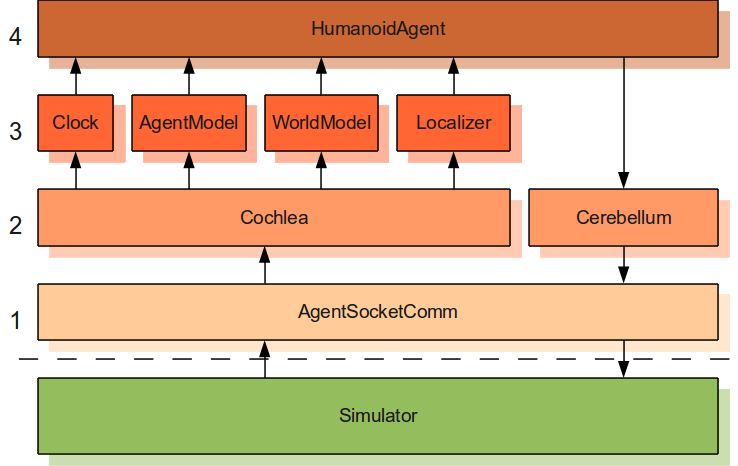
\includegraphics[width=0.7\textwidth]{libbats.png}
	\caption{{\tt libbats} modules}
	\label{fig:libbats}
\end{figure}

The main {\tt libbats} modules and their relations are shown in Fig.~\ref{fig:libbats}. As you can see, they can be divided into several layers:
\begin{description}
\item[1: Low level communication] As discussed in chapter \ref{chSimspark}, communication between the simulator and an agent is done using an ASCII, S-expression based protocol through a TCP/IP connection. The {\tt AgentSocketComm} module handles setting up this connection, reading and writing messages, and parsing these messages into and from more managable data structures. 
\item[2: Input and output integration] In the second layer, input and output is handled at a slightly higher level. On the input side, the {\tt Cochlea} extracts all data from the still text-based messages supplied by the {\tt AgentSocketComm} and turns that data into readily usable binary values. The {\tt Cerebellum} is used to gather control commands, work out contradictions if necesary and turn them into the text based structures that the {\tt AgentSocketComm} understands.
\item[3: Models] The 4 modules in the third layer use the data from the {\tt Cochlea} to update models of the current state of the world, i.e. the current time, the state of the agent's body, the state of the world and the game, and the location of all objects in the field.
\item[4: Intelligence] Finally, at the highest level, the actual intelligence of the agent is implemented. An instance of {\tt HumanoidAgent} has access to all information gathered in the different modules, decides upon actions based on this information, and submits these actions to the {\tt Cerebellum}.
\end{description}

In the following sections we will describe in more detail how each module can be used. While doing so, we will encounter different helper and utility classes. Please refer to later chapters for more details on these. Also, again, for more information, make sure to read the Doxygen documentation contained in the source.

\lstset{numbers=none}

\section{AgentSocketComm}
\label{secSocketComm}

\lstset{numbers=none}

As mentioned earlier, the lowest layer in the library manages the communication with the simulation server. This communication is done through TCP sockets and consists of S-expressions (predicates) that the agent and server send back and forth. To make sure you don't have to worry about what this stuff actually is and does, the library offers you the {\tt AgentSocketComm}. This class handles the connection to the server and sending, receiving and parsing of messages. This section explains how to use this module. If you use the {\tt HumanoidAgent} class, all this is done for you.

Before you can use {\tt AgentSocketComm}, you have to supply a host name and a port number to connect to. When running the server on the same computer as your agent, with default settings, these are 'localhost' and '3100'. After this is done, the first thing to do is to open an actual connection by calling {\tt connect()}:
\begin{lstlisting}[frame=single]
AgentSocketComm& comm = SAgentSocketComm::getInstance();
comm.initSocket("localhost", 3100);
comm.connect();
\end{lstlisting}

Note that the {\tt AgentSocketComm} is a singleton, refer to later chapters for information on what this is. The {\tt AgentSocketComm} keeps two internal message queues, one for input and one for output. These queues are filled and emptied, respectively, when calling {\tt AgentSocketComm}'s {\tt update()} method. This call blocks until new data is received from the server:
\begin{lstlisting}[frame=single]
comm.update();
\end{lstlisting}

SocketComm supplies several methods to place messages that should be sent to the server into the output queue. First of all, you can build your own predicate using the {\tt Predicate} and/or {\tt Parser} classes \footnote{This method is not described in this manual. Look at the documentation of the respective classes for more info} and put it directly into the queue by calling the send method:
\begin{lstlisting}[frame=single]
rf<Predicate> myPredicate = makeMyPredicate();
comm.send(myPredicate);
\end{lstlisting}
However, you can also leave the trouble of building the predicates to {\tt AgentSocketComm} by using its {\tt make*Message()} methods. And if you want it totally easy, use the {\tt init()}, {\tt beam()} and {\tt move*()} methods, which not only build the predicates, but also place the messages directly into the queue for you.

The input queue holds the messages received from the server. To check whether there is a new message, you can call {\tt hasNextMessage}. To extract the next message, you can use {\tt nextMessage()}:
\begin{lstlisting}[frame=single]
while (comm.hasNextMessage())
  rf<Predicate> message = comm.nextMessage();
\end{lstlisting}

To conclude and summarize this section, a typical way to have successful communication with the server is presented here:
\begin{lstlisting}[frame=single]
// Get the AgentSocketComm, initialize and connect
AgentSocketComm& comm = SAgentSocketComm::getInstance();
comm.initSocket("localhost", 3100);
comm.connect();

// Create robot model
rf<Predicate> scene = new Predicate("scene");
scene->pushLeaf("rsg/agent/" + am.getRSG());
comm.send(scene);

// Wait for the first message from the server
comm.update();

// Identify yourself to the server
comm.init(0, "MyTeam");

// Main loop
while (true)
{
  comm.update();
  while (comm.hasNextMessage())
    handleMessage(comm.nextMessage());
}
\end{lstlisting}

\section{Cochlea}
\label{secCochlea}

\lstset{numbers=none}

The {\tt AgentSocketComm} parses the S-expressions that the agent receives from the server into a {\tt Predicate} structure. However, to extract useful data you still have to dig through these structures. The {\tt Cochlea} offers a layer over the {\tt AgentSocketComm} to extract information from the predicates received from the server and present it in an easily accessible way.

Before using the Cochlea you have to initialize some parameters. You have to let it know what the name of your team is, so it can tell team mates and opponents apart:
\begin{lstlisting}[frame=single]
Cochlea& cochlea = SCochlea::getInstance();
cochlea.setTeamName("MyTeam");
\end{lstlisting}

Next you have to set up translations for joint-angle sensors. The {\tt Cochlea} uses internal names for these, that may not be the same as the names used in the messages sent by the server. These internal names are "head1", "head2", "larm1" to "larm4" for the left arm, "rarm1" to "rarm4" for the right and "lleg1" to "lleg6" and "rleg1" to "rleg6" for the legs. The Nao robot used by the server for instance uses names of the form "laj1" and "rlj3", so these have to be translated:
\begin{lstlisting}[frame=single]
cochlea.setTranslation("laj1", "larm1");
cochlea.setTranslation("rlj3", "rleg3");
\end{lstlisting}
This way the Cochlea can handle different robot models. If you use the {\tt AgentModel} module, this is done for you.

Now you can start using the {\tt Cochlea} by calling {\tt update()} every time a new message is received by the {\tt AgentSocketComm}. This will integrate the information of the message, after which you can request data with the {\tt getInfo()} method, or one of the methods for more complex data:
\begin{lstlisting}[frame=single]
comm.update();
cochlea.update();
// Get the polar coordinates of the ball
Vector3D polarBallPos = cochlea.getInfo(
                          Cochlea::iVisionBall);
\end{lstlisting}

\section{Clock}
\label{secClock}

The {\tt Clock} is pretty straightforward: it tells the current time:
\begin{lstlisting}[frame=single]
double t = SClock::getInstance().getTime()
\end{lstlisting}

\section{AgentModel}
\label{secAgentModel}

The \\{\tt AgentModel} keeps a model of the agent's own state. It keeps track of joint angles and data of other sensors, as well as some higher level data, like the position of the Center Of Mass (COM). The {\tt AgentModel} also needs some initialization before it can be used. You have to tell it the uniform number of the agent, after which you should call the {\tt initBody()} method:
\begin{lstlisting}[frame=single]
AgentModel& am = SAgentModel::getInstance();
am.setUnum(unum);
am.initBody();
\end{lstlisting}

This loads an XML configuration file that contains the names, sizes and weights of the agent's body parts and joints. It also uses this data to set up the translations for the {\tt Cochlea} for you, so you don't have to do this by hand. If default settings are used, the default configuration file {\tt conf.xml} is loaded, which is installed with the library and which imports the {\tt nao\_mdl.xml} file for each agent to get the description of the Nao robot model. For more information on loading XML configuration files and the robot model descriptions, see the documentation of the {\tt Conf} class.

After initialization, the {\tt AgentModel} is also ready to be updated and used:
\begin{lstlisting}[frame=single]
comm.update();
cochlea.update();
am.update();

Vector3D com = am.getCOM();
\end{lstlisting}

\section{WorldModel}
\label{secWorldModel}

The raw data offered by the {\tt Cochlea} may not be directly usable and perhaps you want to have some information that is deduced from these facts. This is exactly what the {\tt WorldModel} is for. It for instance gives the current game state and field size, but also higher level information like which team should take the kick-off, or if there is another player closer to the ball.

To start, the {\tt WorldModel} also needs to know the name of your team for some of its capabilities:
\begin{lstlisting}[frame=single]
WorldModel& wm = WorldModel::getInstance();
wm.setTeamName("MyTeam");
\end{lstlisting}

Next, the model has to be updated at every cycle. The {\tt WorldModel} extracts data from the {\tt Cochlea}, so make sure it is updated before updating the {\tt WorldModel}:
\begin{lstlisting}[frame=single]
comm.update();
cochlea.update();
wm.update();

bool shouldWeKickOff = wm.weGetKickOff();
\end{lstlisting}

\section{Localizer}
\label{secLocalizer}

\begin{figure}
\centering
\subfigure[Agent]{
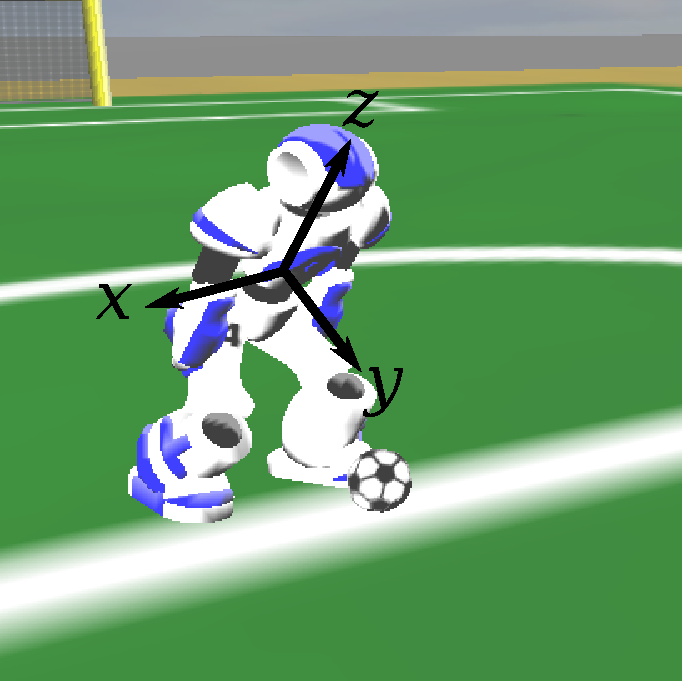
\includegraphics[width=.3\textwidth]{raw.pdf} \label{coordinatesraw}
}
\subfigure[Local]{
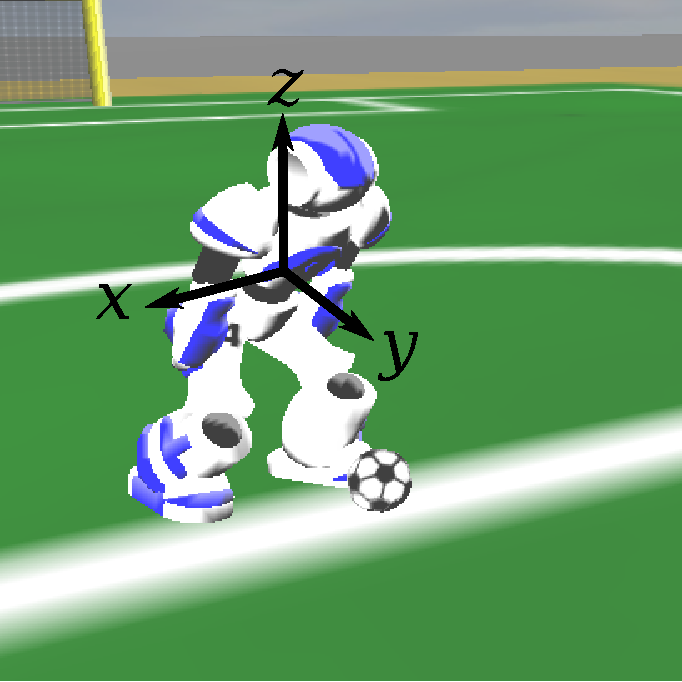
\includegraphics[width=.3\textwidth]{local.pdf} \label{coordinateslocal}
}
\subfigure[World]{
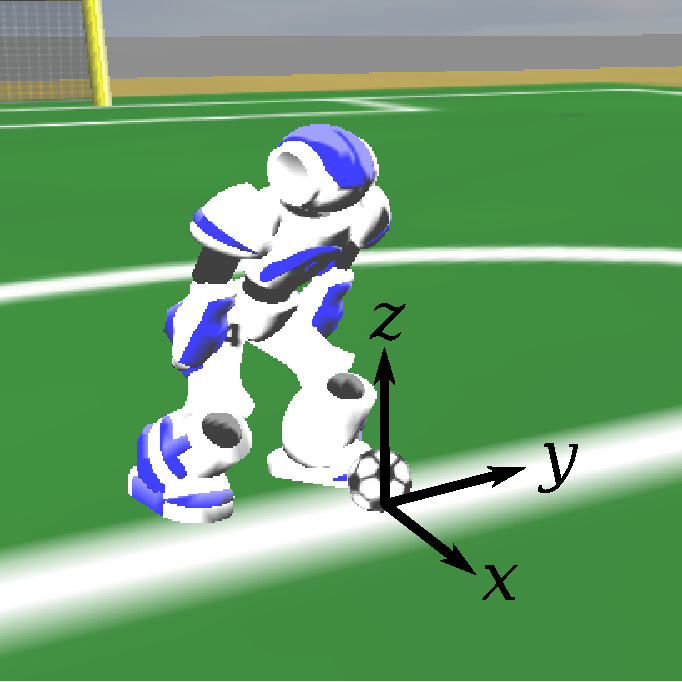
\includegraphics[width=.3\textwidth]{world.pdf}\label{coordinatesworld}
}
\caption{The coordinate systems used in {\tt libbats}: (a) Agent ('raw') coordinates, (b) local coordinates, and (c) global coordinates.}
\label{coordinates}
\end{figure}

The WorldModel provides the state of the game, such as the game time, the gamestate, and the team name. However, often the agents will want to know where they are, where the ball is, or where their opponents are. This can be obtained through the {\tt Localizer}. To be able to implement different localization methods, the {\tt Localizer} is an abstract class from which all implementations are derived. One realization of this class is provided in {\tt libbats}, called the {\tt KalmanLocalizer}. As you might have guessed, this {\tt Localizer} uses a Kalman filter to keep track of the locations of the player itself and of other objects. At the start of the program, we have to initialize the Localizer and tell it which implementation to use:
\begin{lstlisting}[frame=single]
SLocalizer::initialize<KalmanLocalizer>();
\end{lstlisting}

Like the other models, the update() member function of the {\tt Localizer} should be called each timestep to update the current location estimates with new data from the {\tt Cochlea}. The other member functions of the Localizer can be used to obtain the current position of the agent itself, the ball, the other players, or objects such as the goal posts and corner flags.

Within {\tt libbats}, several different coordinate systems are used (see Fig.~\ref{coordinates}:
\begin{description}
\item[Agent/raw coordinates] The origin of this system is the center of the agent's torso. The positive x axis extends to the right, parallel to the line through the shoulders, the positive y axis forward out of the torso, and the positive z-axis upwards, through the center of the head. This system is used by the {\tt AgentModel} for the coordinates of body parts. Shown in Fig.\ref{coordinatesraw}.
\item[Local coordinates] The origin of the local coordinate system is also the center of the agent's torso, but the positive z axis of this system always points upwards, perpendicular to the field. So, the x and y axes always lie parallel to the field, pointing right and forward respectively. This is one of the systems used by the {\tt Localizer} and is the most intuitive to use to determine 'in front of me/to the side of me/above of me' relations. Shown in Fig.\ref{coordinateslocal}.
\item[World coordinates] The world coordinate system is fully independent of the agent's location and orientation. Its origin is the center of the field, the positive x axis points to the center of the opponent's goal, the positive y-axis to the left when looking along the x axis, and the positive z axis points up, perpendicular to the field. This is the second system that is used by the {\tt Localizer} and is the best one to use to determine global relations. Shown in Fig.\ref{coordinatesworld}.
\end{description}

\section{Cerebellum}
\label{secCerebellum}

The {\tt Cochlea} takes the trouble of having to deal with raw predicates on the input side. On the output side the {\tt Cerebellum} is there for you. It supplies more useful structures to define actions and the possibility to integrate actions from different sources in your agent. The {\tt Cerebellum} defines the {\tt Action} substructure and a few of its derivatives with which you can make new actions. At the moment there are 5 different action types available:
\begin{description}
\item[{\tt MoveJointAction}] Move a hinge joint or one axis of a universal joint.
\item[{\tt MoveHingeJointAction}] Move a hinge joint.
\item[{\tt MoveUniversalJointAction}] Move both axes of a universal joint.
\item[{\tt BeamAction}] Beam to a certain position.
\item[{\tt SayAction}] Shout something.
\end{description}
If you don't understand the difference between hinge and universal joints, don't worry. Just use {\tt MoveJointAction}s and let the {\tt Cerebellum} handle the rest.

The {\tt Cerebellum} again is a singleton that can be retrieved by calling \\ {\tt SCerebellum::getInstance()}, after which you can add actions to it. After all the sub parts have added their actions, you can call {\tt outputCommands()} to send them through an {\tt AgentSocketComm}:
\begin{lstlisting}[frame=single]
Cerebellum& cer = SCerebellum::getInstance();

rf<MoveJointAction> action =
  new MoveJointAction(Types::LLEG1, 0.1);
cer.addAction(action);

cer.outputCommands(comm);
\end{lstlisting}
When more than one action is supplied for a joint, the angular velocities will be added together before sending the actions to the server.

\section{HumanoidAgent}
\label{secHumanoidAgent}

Now you have learned about how to initialize, update and maintain the several models of the library, you will learn how to forget all that. The {\tt HumanoidAgent} class does this all for you. It connects the {\tt AgentSocketComm}, initializes the {\tt Clock}, {\tt AgentModel}, {\tt WorldModel} and {\tt Localizer} and updates all modules in the correct order at every cycle. See chapter \ref{chQuickstart} to learn how to use this class to set up your own agent.

%\section{Behavior}
%\label{secBehavior}
%
%The code in the previous section implements an agent which connects to te server, gets placed in the field and then stands there until it falls over. Now it is time to let your agent behave. The BATS agent architecture supplies a hierarchical behavior model to help you with this by following these steps:
%
%\begin{itemize}
%\item Implement seperate behaviors
%\item Create a configuration file placing the behaviors in a hierarchical structure
%\item Create and run the behaviors
%\end{itemize}
%
%\subsection{Implementing a behavior}
%\label{subsecImplementingBehavior}
%
%The BATS agent architecture gives the {\tt Behavior} class as the building block of your agent. The basic thing to know is that a behavior receives a goal from a higher level behavior, creates subgoals that it wants to achieve in order to achieve the main goal and passes these goals to its subbehaviors. The behavior defines a sequence of slots in which arbitrary sub behaviors can be placed. This section shows how to create a behavior, section \ref{subsecConfiguration} will show how to define its super and sub behaviors.
%
%\subsubsection*{Inherit Behavior}
%
%The first thing to do when creating a new behavior is to create a class that inherits from the {\tt Behavior} class. It defines a couple of pure virtual methods that each behavior should implement (more on these later):
%
%\begin{program}
%\begin{verbatim}
%class MyBehavior : public Behavior
%{
%  virtual rf<Goal> generateGoal(unsigned step,
%                                unsigned slot);
%  virtual rf<State> getCurrentState();
%  virtual ConfidenceInterval getCapability(rf<State> s,
%                                           rf<Goal> g);
%
%public:
%  MyBehavior(std::string const &id,
%             std::string const &playerClass);
%};
%\end{verbatim}
%\end{program}
%
%You can do this by hand, but you can also use the utility script {\tt createbehavior.pl} to do this for you:
%
%\begin{program}
%\begin{verbatim}
%$ cd util/
%$ ./createbehavior.pl
%[Enter the behaviors name (e.g. MyBehavior)]
%\end{verbatim}
%\end{program}
%
%This creates a directory with your behavior's name in the Behavior directory and fills it with a header file with the necesary method declarations and code files with basic implementations for these methods.
%
%\subsubsection{Constructor (defining slots)}
%
%After making the base of your behavior you have to implement the constructor, where you define the structure of the behavior's sub behaviors by creating slots. The {\tt createbehavior.pl} script makes a start by creating a tree that defines a sequence of 1 step with 1 slot:
%
%\begin{program}
%\begin{verbatim}
%// Define the root, which is always a sequence:
%d_tree = new AST::Node(sequenceType);
%// Add one step to the sequence:
%d_tree->addChild(new AST::Node(andType));
%// Add one slot to the first step:
%d_tree->getChild(0)->addChild(new AST::Node(orType));
%\end{verbatim}
%\end{program}
%
%If you need more steps in the sequence, you can add new conjunction nodes ({\tt andType}) to the root, if you want to run sub behaviors in parallel in a step, you can add new disjunction nodes ({\tt orType}). The following gives an example of a behavior with 3 sequence steps and 2 parallel slots in the second step:
%
%\begin{program}
%\begin{verbatim}
%// Define the root, which is always a sequence:
%d_tree = new AST::Node(sequenceType);
%
%// Add first step to the sequence:
%d_tree->addChild(new AST::Node(andType));
%// Add one slot to the first step:
%d_tree->getChild(0)->addChild(new AST::Node(orType));
%
%// Add second step to the sequence:
%d_tree->addChild(new AST::Node(andType));
%// Add two slots to the second step:
%d_tree->getChild(1)->addChild(new AST::Node(orType));
%d_tree->getChild(1)->addChild(new AST::Node(orType));
%
%// Add third step to the sequence:
%d_tree->addChild(new AST::Node(andType));
%// Add one slot to the third step:
%d_tree->getChild(2)->addChild(new AST::Node(orType));
%\end{verbatim}
%\end{program}
%
%\subsubsection*{getCurrentState()}
%
%The first virtual method to implement is {\tt getCurrentState}. Different behaviors rely on different information of the world and/or agent state. In the BATS agent architecture a behavior defines this state itself in a standardized tree-based state description. This standardization is useful when using a learning algorithm to train different behaviors that use different state information. These state descriptions can also be used to define goals as states that should be reached, as we will see in the next sections.
%
%A basic state description is a conjunction of the state of several variables. To cater for uncertainty, the state of a variable is defined as a range of possible values:
%
%\begin{equation}
%\label{eqState}
%(0 \leq BallDist < 5) \wedge (10 \leq OpponentDist < 15)
%\end{equation}
%
%A behavior's state is defined in its {\tt getCurrentState} method. The {\tt createbehavior.pl} script sets up a conjunction for you to place variables into. The following code shows how to create the state in \ref{eqState}:
%
%\begin{program}
%\begin{verbatim}
%rf<State> state = new State();
%rf<OrNode> dis = state->addDisjunct();
%rf<AndNode> con = dis->addConjunct();
%
%con->addVar("BallDist", 0, 5);
%con->addVar("OpponentDist", 10, 15);
%\end{verbatim}
%\end{program}
%
%
%\subsubsection*{getCapability()}
%
%Behaviors that are placed in the same slot compete with each other for execution. They receive the same goal and are selected based on their capability to achieve that goal. Also, before advancing to the next sequence step, a behavior checks whether the sub behaviors in that step have enough capability to finish that step. A behavior's capability is requested by calling its {\tt getCapability} method, passing it a goal and the state it created in {\tt getCurrentState}. The behavior returns an estimate of its capability of achieving the goal, ranging from -1 to 1, with a confidence interval that depicts the accuracy of the estimate.
%
%\subsubsection*{Commitment}
%
%As explained earlier a behavior can commit to its goal when it is chosen. By doing so, it lets the super behavior know that it will take some time to reach the goal and that in intermediate steps it could not be good to switch between behaviors. Commitment is requested by setting the d\_committed member variable, which should be done in the behavior's overloaded {\tt update} method:
%
%\begin{program}
%\begin{verbatim}
%void MyBehavior::update()
%{
%  Behavior::update();
%  
%  // Check if we are already committed
%  // due to committed subbehavior(s)
%  if (d_committed)
%    return;
%  
%  // Commit if we can still reach our goal  
%  if (goalStillReachable())
%    d_committed = true;
%  else
%    d_committed = false;
%\end{verbatim}
%\end{program}
%
%The {\tt update} method is called at the beginning of each time step if the behavior could be selected to run that timestep. First of all the {\tt Behavior::update} should be called. This updates the child behaviors, checks if they are committed and commits the behavior if it should commit if children are committed \footnote{Abbreviated to SCICC (Should Commit If Children Commit)}. If this is the case you can choose to override this, but usually you just return.
%
%Next you check whether the behavior should commit to its goal. Usually this is the case when the goal can still be reached. It is important to also reset the flag when a goal is no longer reachable, as shown in the example, to prevent a behavior to lock the agent in useless behavior. Note that the behavior's goal ({\tt d\_goal}) is the goal received in the previous timestep.


%\subsection{Configuration XML setup}
%\label{subsecConfiguration}
%The humanoidbats agent has to have an XML configuration file. This file is used to structure all the behaviors in the binary together. The XML file will define all the steps and slots and will define a root behavior which is at the top of the behavior hierarchy.
%The general XML layout contains:
%%
%%
%%  HIERONDER MNOETEN NOG LINKS KOMEN NAAR DE HOOFDSTUKKEN..........
%%
%%
%%
%\begin{itemize}
%\item The root conf element
%	\item The player id (unum) to class type coupling
%	\item The player class defenitions
%\begin{itemize}
%		\item The behaviors element
%\begin{itemize}
%			\item Behavior elements
%\begin{itemize}
%				\item Behavior parameters
%				\item Behavior slots
%\end{itemize}
%\end{itemize}
%\end{itemize}
%\item XIncludes
%\end{itemize}
%
%\subsubsection*{The root conf element}
%Every XML file has a root element, in the configuration XML files this is the conf element. If the file includes other XML files, make sure to include the XInclude namespace. The most common header will therefore contain:
%
%\begin{program}
%\begin{verbatim}
%<?xml version="1.0" encoding="ISO-8859-1"?>
%
%<conf xmlns:xi="http://www.w3.org/2003/XInclude">
%\end{verbatim}
%\end{program}
%
%
%\subsubsection*{The player id (unum) to class type coupling}
%All the players on the field share the same XML configuration files as they are all instances of the same command. To allow for the different player types to share the same XML, the playerclass has been added. Every agent has a playerclass, and all player classes have their own behavior hierarchy. To define which player class is used for which unum, the following code is used:
%
%\begin{program}
%\begin{verbatim}
%<player id="1" class="attacker" />
%\end{verbatim}
%\end{program}
%
%
%\subsubsection*{The player class definitions}
%The player class element holds the behaviors for the player class. Every player class has an id and contains the behaviors.
%
%\begin{program}
%\begin{verbatim}
%<player-class id="attacker">
%\end{verbatim}
%\end{program}
%
%\subsubsection*{The behaviors element}
%The behaviors element is a simple container element for all the behavior elements. It currently has no attributes, but must contain at least one behavior with the id “win”.
%
%\subsubsection*{Behavior elements}
%The behavior elements contain all the information for the behavior structure. Every behavior has a type, that names the name of the behavior in the binary, and an unique id, which is used to reference it from other parts of the XML. The id only has to be unique within the behaviors parent element, not the whole configuration XML.
%
%\begin{program}
%\begin{verbatim}
%<behavior type="MyBehavior" id="mybehavior">
%\end{verbatim}
%\end{program}
%
%\subsubsection*{Behavior parameters}
%Behavior parameters are behavior specific and are used in by the binary behavior to make it more general in use.
%All parameters for a behavior are kept inside the \emph{param} element. This element can contain any type of element which is totally up to the binary behavior.
%An example of is:
%\begin{program}
%\begin{verbatim}
%  <param>
%        <deg>10</deg>
%        <joint slot="0">&rleg5;</joint>
%        <joint slot="1">&lleg5;</joint>
%  </param>
%\end{verbatim}
%\end{program}
%
%\subsubsection*{Behavior slots}
%Every behavior can have other behaviors below it. These other behaviors can be run in parallel, in sequence, or in competition.
%The slots are created with a \emph{slot} element which is a direct descendant of the behavior element. Each slot has an index attribute
%which describes where it is placed below the behavior. The first digit of the index indicates the step, and the second digit indicates the slot. Each slot, in turn, contains any number of references to behaviors defined in the
%configuration.
%
%Remember, steps are executed in sequence. Within steps, slots are executed in parallel, and within each slot only one of the alternative behaviors is chosen.
%
%To reference to a behavior, a \emph{behavior} element should be used with a \emph{refid} attribute containing the XML configuration id of the behavior.
%
%A typical example:
%
%\begin{program}
%\begin{verbatim}
%<slot index="0-0">
%  <behavior refid="alternativeA" />
%  <behavior refid="alternativeB" />
%  <!--either alternativeA or alternativeB is executed -->
%</slot>
%<slot index="0-1">
%  <behavior refid="parallelBehavior" />
%  <!--parallelbehavior is executed in parallel with 
%  either alternativeA or alternativeB-->
%</slot>
%<slot index="1-0">
%  <behavior refid="secondStep" />
%  <!--secondStep is done after all of the above -->
%</slot>
%\end{verbatim}
%\end{program}
%
%
%\subsection{Creating and Running Behaviors}
%
%Now you have defined all your behaviors and set up the hierarchy in your XML configuration file. The last thing to do is to have your agent create the correct behavior tree based on the configuration file and run the behaviors every time step. The first you simply do by loading the configuation file with the {\tt Conf} class and then call the static {\tt Behavior::createBehaviors} method:
%
%\begin{program}
%\begin{verbatim}
%void MyAgent::init()
%{
%  Conf::initialize("myconf.xml");
%  Behavior::createBehaviors();
%}
%\end{verbatim}
%\end{program}
%
%As you can see, your agent's {\tt init} method is a good place to do it. Running your behaviors consists of running the root behavior, which in its turn runs its subbehaviors, et cetera, until the lowest, primitive behaviors are run. Just select your root behavior (we like to call it the 'win' behavior and is the behavior with id 'win') and run it:
%
%\begin{program}
%\begin{verbatim}
%void MyBehavior::think()
%{
%  rf<Behavior> win = Behavior::getWin();
%  win->update();
%  win->setGoal(new Behavior::Goal);
%  win->achieveGoal();
%}
%\end{verbatim}
%\end{program}
%
%After the behavior tree is processed, the primitive behaviors that have actions to send to the server  are collected in the list of Action Command Behaviors. You should request these, collect their actions and send them to the Cerbellum:
%
%\begin{program}
%\begin{verbatim}
%void MyBehavior::think()
%{
%  ...
%  Cerebellum& cer = SCerebellum::getInstance();
%  
%  std::set<rf<Behavior> > acBehaviors = 
%      Behavior::getActionCommandBehaviors();
%  for (set<rf<Behavior> >::iterator iter = 
%          acBehaviors.begin(); iter != acBehaviors.end(); ++iter)
%  	cer.addAction((*iter)->getAction());
%  
%  cer.outputCommands(d_comm);
%}
%\end{verbatim}
%\end{program}


\chapter{Movement}
\label{cha:movement}


%%% Local Variables: 
%%% mode: latex
%%% TeX-master: "libbatsmanual"
%%% End: 

\chapter{Utility Classes}

Next to the main modules described in the previous chapter, {\tt
  libbats} offers a collection of utility classes. We will discuss
these here.

\lstset{numbers=none}

\section{Singleton}
\label{secSingleton}

Many modules of the library are so called singletons, so we will give
a short introduction about what this is and how they are used. The
singleton pattern is a design pattern that makes sure that there is no
more than one instance of a certain class. For instance, there is only
one Queen of The Netherlands, it would make no sense to create
multiple instances. In the singleton design pattern, special measures
are taken to prevent you from copying the single instance or creating
new objects of the class. This pattern is used in the library for
modules for which it makes no sense and for which it could cause
problems if there are multiple instances. This is for instance the
case for modules keeping track of states, such as the {\tt Localizer}
and the {\tt AgentModel}, and a module for maintaining the connection
with the server.

In this library, singletons are implemented by the {\tt Singleton<T>}
template class. It offers the static {\tt getInstance()} method to
request a reference to the single instance of class {\tt T}. For
instance, the following shows how to get a reference to the {\tt
  WorldModel}:
\begin{lstlisting}[frame=single]
WorldModel& wm = Singleton<WorldModel>::getInstance();
\end{lstlisting}
For each singleton class of the library, a {\tt typedef} is set for
the {\tt Singleton<T>} instantiation of that class, formed by
prefixing the class name with a capital S. So another way to write the
previous example would be:
\begin{lstlisting}[frame=single]
WorldModel& wm = SWorldModel::getInstance();
\end{lstlisting}

If you want to use the {\tt Singleton<T>} template to create
singletons of your own class, make sure it adhears to the following
points:
\begin{itemize}
\item Your class must have a default constructor.
\item Make all constructors, including the copy constructor, of your
  class private.
\item Make the assignment operator, {\tt operator=}, private.
\item Define {\tt Singleton<T>}, instantiated with your own class, as
  friend of your class.
\end{itemize}
If you do this, your class definition will look like this:
%\lstset{numbers=left,numberstyle=\small}
\begin{lstlisting}[frame=single]
class MySingleton
{
  friend class bats::Singleton<MySingleton>;
private:
  // Default constructor
  MySingleton() {}
  // Copy constructor, not implemented
  MySingleton{MySingleton const& other);
  // Assignment operator, not implemented
  MySingleton& operator=(MySingleton const& other);
public:
  // Some public stuff
};
// libbats style singleton typedef
typedef bats::Singleton<MySingleton> SMySingleton;
\end{lstlisting}

\section{Distribution}

Agents often have to work with uncertainty and probability
distributions. For instance, vision data received from the simulator
is limited and noisy, therefore location estimates derived from this
data are just that: estimates, with a certain variability. To deal
with this, {\tt libbats} offers the {\tt Distribution} template. This
template supports distributions over any number of dimensions, though
most commonly 1D distributions, e.g. for joint angles, and 3D
distributions, e.g. for locations, are used. Currently there is only a
single implementation of this template, the {\tt NormalDistribution},
however it is possible to create new distribution types, like Monte
Carlo or histogram based representations.

The most common operation on a distribution is to get the mean value,
or 'the most likely' value, which is done with the {\tt getMu()}
method. For instance, when asking the {\tt Localizer} for a location,
it returns a ({\tt rf} to a) 3D distribution, so to get the most
likely local location of the ball you use:
%\lstset{numbers=left,numberstyle=\small}
\begin{lstlisting}[frame=single]
Vector3D ballLoc = localizer.getLocationLocal(Types::BALL)->getMu();
\end{lstlisting}

Other useful methods are {\tt getSigma()}, to get the distribution's
covariance matrix, and {\tt draw()}, to draw a random value from the
distribution:
%\lstset{numbers=left,numberstyle=\small}
\begin{lstlisting}[frame=single]
Matrix3d ballVariance = localizer.getLocationLocal(Types::BALL)->getSigma();
// 1 dimensional normal distribution
rf<Distribution> myDist = new NormalDistribution(1)
// Initialize distribution with mean 0 and variance 1
Vector1d mu = Vector1d::Zero();
Matrix1d sigma = Matrix1d::Ones();
myDist->init(mu, sigma);
// Draw a random value
Vector3d v = myDist->draw();
\end{lstlisting}

\section{Math}
Several common mathematical problems that are useful in 3D Soccer
Simulation are included in {\tt libbats} as methods of the {\tt Math}
class. Some of these are pretty selfexplenatory, for the rest see the
following descriptions (and again the documentation in the code
itself):

\begin{tabular}{l l}
\begin{minipage}{0.7\textwidth}
\begin{description}
\item[distanceLinePoint] This method is used to calculate the distance
  between a line and a point. The line, dashed black in the example to
  the right, is defined by a point vector $l_0$ and a direction vector
  $\vec{l}$, the point $p$ is also a point vector. The method returns
  the length of the red, dotted line $d$.
\end{description}
\end{minipage}
&
\begin{minipage}{0.3\textwidth}
  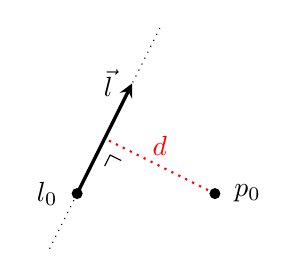
\begin{tikzpicture}[scale=.7]
    \draw[dotted] (0,0) -- (2,4);
    \node[label=left:$l_0$] (lz) at (0.5,1) {};
    \node[label=left:$\vec{l}$] (ld) at (1.5,3) {};
    \node[label=right:$p_0$] (p0) at (3,1) {};
    \node[] (p1) at (1,2) {};

    \draw[very thick,->,>=stealth] (lz.center) -- (ld.center);
    \draw[dotted,thick,red] (p0.center) -- node[above]{$d$} (p1.center);
    \fill (lz) circle(0.1);
    \fill (p0) circle(0.1);
    
    \draw ($(p1.center) + (0.0,-0.5)$) -- ++(0.1,0.2) -- ++(0.2,-0.1);
  \end{tikzpicture}
\end{minipage}
\end{tabular}

\begin{tabular}{l l}
\begin{minipage}{0.7\textwidth}
\begin{description}
\item[linePointClosestToPoint] This method is used to determine the
  point on a line that is closest to a given point. The line, dashed
  black in the example to the right, is defined by a point vector
  $l_0$ and a direction vector $\vec{l}$, the point $p_0$ is also a
  point vector. The method returns the coordinates of point $p_1$.
\end{description}
\end{minipage}
&
\begin{minipage}{0.3\textwidth}
  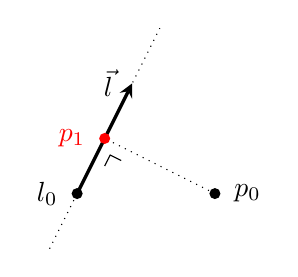
\begin{tikzpicture}[scale=.7]
    \draw[dotted] (0,0) -- (2,4);
    \node[label=left:$l_0$] (lz) at (0.5,1) {};
    \node[label=left:$\vec{l}$] (ld) at (1.5,3) {};
    \node[label=right:$p_0$] (p0) at (3,1) {};
    \node[label=left:\color{red}$p_1$] (p1) at (1,2) {};

    \draw[very thick,->,>=stealth] (lz.center) -- (ld.center);
    \draw[dotted] (p0.center) -- (p1.center);
    \fill (lz) circle(0.1);
    \fill (p0) circle(0.1);
    \fill[red] (p1) circle(0.1);
    
    \draw ($(p1.center) + (0.0,-0.5)$) -- ++(0.1,0.2) -- ++(0.2,-0.1);
  \end{tikzpicture}
\end{minipage}
\end{tabular}

\begin{tabular}{l l}
\begin{minipage}{0.7\textwidth}
\begin{description}
\item[intersectVectorPlane] Determine the coordinates of the
  intersection of a line with a plane. The line, dashed black in the
  example to the right, is defined by a point vector $l_0$ and a
  direction vector $\vec{l}$. The plane is defined by the vector $(a,
  b, c, d)^T$, such that $ax + by + cz = d$. In this representation,
  the vector $(a,b,c)^T$ is normal to the plane and $d$ is the
  distance of the plane to the origin of the reference frame. The
  method returns the coordinates of point $p$.
\end{description}
\end{minipage}
&
\begin{minipage}{0.3\textwidth}
  \begin{tikzpicture}[scale=.7]
    \draw[dotted] (1.25,0) -- (1.75,1);
    \fill[Cerulean!30!white] (-0.5,1) -- (0.5,2) -- (4.5,2) -- (3.5,1);
    \draw[dotted,Cerulean!70!black] (1.75,1) -- (2,1.5);
    \draw[dotted] (2,1.5) -- (3,3.5);
    
    \node[label=right:\color{red}$p$] (p) at (2,1.5) {};
    \fill[red] (p) circle(0.1);
    
    \node[label=left:$l_0$] (lz) at (2.4,2.3);
    \node[label=left:$\vec{l}$] (ld) at (2.9,3.3);

    \draw[very thick,->,>=stealth] (lz.center) -- (ld.center);
    \fill (lz) circle(0.1);
  \end{tikzpicture}
\end{minipage}
\end{tabular}

\section{Types}

The {\tt Types} class holds many useful types and enumerations, used
throughout the library. Here is a brief overview of these, but also
make sure to look at the code documentation.
\begin{description}
\item[PlayMode] This enumeration list all the possible play modes. For
  modes of which there are two side variants, e.g. kick-off and free
  kick, there is also an 'us' and a 'them' version. It is recommended
  to use these instead of the left/right versions, and all {\tt
    libbats} modules use the us/them versions. For instance, if the
  left team gets the kick-off, and our team plays on the right, {\tt
    WorldModel::getPlayMode()} will return {\tt Types::KICKOFF\_THEM}.
\item[Side] A simple enumeration to discern left and right in a
  human-readable manner.
\item[Joint] An enumeration of all the agent's joints. This is for
  instance used to get the current angle of a joint from the {\tt
    AgentModel}:
\begin{lstlisting}[frame=single]
  // Get angle of the first joint of the left arm, in radians double
  angle = am.getJoint(Types::LARM1)->angle.getMu()(0);
\end{lstlisting}
\item[BodyPart] An enumeration of all the agent's body parts. This is
  for instance used to get the current location of a body part from
  the {\tt AgentModel}:
\begin{lstlisting}[frame=single]
// Get the position of the left foot, relative to the torso
Vector3d pos = am.getBodyPart(Types::LFOOT)->transform.translation;
\end{lstlisting}
\item[Object] This enumeration lists all objects in the environment,
  such as the ball, players, opponents, and landmarks. For the latter
  there are left/right and us/them versions. Again, it is recommended
  to use the us/them variants:
\begin{lstlisting}[frame=single]
// Get the location of the first post of the opponent goal,
// in local coordinates
Vector3d pos = localizer.getLocaltionLocal(Types::GOAL1THEM)->getMu();
\end{lstlisting}
\end{description}

%%% Local Variables: 
%%% mode: latex
%%% TeX-master: "libbatsmanual"
%%% End: 



%\appendix

%\chapter{List of joints}
\begin{tabular}{ll}
\&head1; & Torso to head, Z-Axis (left/right)\\
\&head2; & Torso to head, X-Axis (up/down)\\
\\
\&lleg1; & Torso to left hip, Z-Axis (twist left/right)\\
\&lleg2; & Left hip to Left thigh, X-Axis (backward/forward)\\
\&lleg3; & Left hip to Left thigh, Y-Axis (spread/close)\\
\&lleg4; & Left thigh to Left shank, X-Axis (stretch/bend)\\
\&lleg5; & Left shank to Left foot, X-Axis (toes down/toes up)\\
\&lleg6; & Left shank to Left foot, Y-Axis (left/right)\\
\\         
\&rleg1; & Torso to right hip, Z-Axis  (twist left/right)\\
\&rleg2; & Right hip to Right thigh, X-Axis (backward/forward)\\
\&rleg3; & Right hip to Right thigh, Y-Axis (spread/close)\\
\&rleg4; & Right thigh to Right shank, X-Axis (bend/stretch)\\
\&rleg5; & Right shank to Right foot, X-Axis (toes down/toes up)\\
\&rleg6; & Right shank to Right foot, Y-Axis (left/right)\\
\\     
\&larm1; & Torso to Left shoulder, X-Axis (forward/backward)\\
\&larm2; & Torso to Left shoulder, Y-Axis (out/in)\\
\&larm3; & Left shoulder to Left upper arm, Z-Axis (twist left/right)\\
\&larm4; & Left upper arm to Left lower arm, X-Axis\\
\\     
\&rarm1; & Torso to Right shoulder, X-Axis (forward/backward)\\
\&rarm2; & Torso to Right shoulder, Y-Axis (out/in)\\
\&rarm3; & Right shoulder to Right upper arm, Z-Axis (twist left/right)\\
\&rarm4; & Right upper arm to Right lower arm, X-Axis\\

\end{tabular}


%\chapter{Behavior overview BATS 2007}
%plaatje van dobehave


\backmatter
%\begin{thebibliography}{}
%
%
%\bibitem{homepage} The Little Green BATS homepage, \\
%    \url{http://www.littlegreenbats.nl/}.
%\bibitem{simspark} Simspark, \\
%    \url{http://simspark.sourceforge.net/}.
%\bibitem{rcssserver3d} RoboCup 3D Simspark Simulation Server (includes 2D server),\\
%    \url{http://sserver.sourceforge.net/}
%
%
%\end{thebibliography}



\end{document}
